% Options for packages loaded elsewhere
\PassOptionsToPackage{unicode}{hyperref}
\PassOptionsToPackage{hyphens}{url}
%
\documentclass[
]{article}
\usepackage{amsmath,amssymb}
\usepackage{lmodern}
\usepackage{ifxetex,ifluatex}
\ifnum 0\ifxetex 1\fi\ifluatex 1\fi=0 % if pdftex
  \usepackage[T1]{fontenc}
  \usepackage[utf8]{inputenc}
  \usepackage{textcomp} % provide euro and other symbols
\else % if luatex or xetex
  \usepackage{unicode-math}
  \defaultfontfeatures{Scale=MatchLowercase}
  \defaultfontfeatures[\rmfamily]{Ligatures=TeX,Scale=1}
\fi
% Use upquote if available, for straight quotes in verbatim environments
\IfFileExists{upquote.sty}{\usepackage{upquote}}{}
\IfFileExists{microtype.sty}{% use microtype if available
  \usepackage[]{microtype}
  \UseMicrotypeSet[protrusion]{basicmath} % disable protrusion for tt fonts
}{}
\makeatletter
\@ifundefined{KOMAClassName}{% if non-KOMA class
  \IfFileExists{parskip.sty}{%
    \usepackage{parskip}
  }{% else
    \setlength{\parindent}{0pt}
    \setlength{\parskip}{6pt plus 2pt minus 1pt}}
}{% if KOMA class
  \KOMAoptions{parskip=half}}
\makeatother
\usepackage{xcolor}
\IfFileExists{xurl.sty}{\usepackage{xurl}}{} % add URL line breaks if available
\IfFileExists{bookmark.sty}{\usepackage{bookmark}}{\usepackage{hyperref}}
\hypersetup{
  pdftitle={Assignment 1},
  pdfauthor={10179889},
  hidelinks,
  pdfcreator={LaTeX via pandoc}}
\urlstyle{same} % disable monospaced font for URLs
\usepackage[margin=1in]{geometry}
\usepackage{color}
\usepackage{fancyvrb}
\newcommand{\VerbBar}{|}
\newcommand{\VERB}{\Verb[commandchars=\\\{\}]}
\DefineVerbatimEnvironment{Highlighting}{Verbatim}{commandchars=\\\{\}}
% Add ',fontsize=\small' for more characters per line
\usepackage{framed}
\definecolor{shadecolor}{RGB}{248,248,248}
\newenvironment{Shaded}{\begin{snugshade}}{\end{snugshade}}
\newcommand{\AlertTok}[1]{\textcolor[rgb]{0.94,0.16,0.16}{#1}}
\newcommand{\AnnotationTok}[1]{\textcolor[rgb]{0.56,0.35,0.01}{\textbf{\textit{#1}}}}
\newcommand{\AttributeTok}[1]{\textcolor[rgb]{0.77,0.63,0.00}{#1}}
\newcommand{\BaseNTok}[1]{\textcolor[rgb]{0.00,0.00,0.81}{#1}}
\newcommand{\BuiltInTok}[1]{#1}
\newcommand{\CharTok}[1]{\textcolor[rgb]{0.31,0.60,0.02}{#1}}
\newcommand{\CommentTok}[1]{\textcolor[rgb]{0.56,0.35,0.01}{\textit{#1}}}
\newcommand{\CommentVarTok}[1]{\textcolor[rgb]{0.56,0.35,0.01}{\textbf{\textit{#1}}}}
\newcommand{\ConstantTok}[1]{\textcolor[rgb]{0.00,0.00,0.00}{#1}}
\newcommand{\ControlFlowTok}[1]{\textcolor[rgb]{0.13,0.29,0.53}{\textbf{#1}}}
\newcommand{\DataTypeTok}[1]{\textcolor[rgb]{0.13,0.29,0.53}{#1}}
\newcommand{\DecValTok}[1]{\textcolor[rgb]{0.00,0.00,0.81}{#1}}
\newcommand{\DocumentationTok}[1]{\textcolor[rgb]{0.56,0.35,0.01}{\textbf{\textit{#1}}}}
\newcommand{\ErrorTok}[1]{\textcolor[rgb]{0.64,0.00,0.00}{\textbf{#1}}}
\newcommand{\ExtensionTok}[1]{#1}
\newcommand{\FloatTok}[1]{\textcolor[rgb]{0.00,0.00,0.81}{#1}}
\newcommand{\FunctionTok}[1]{\textcolor[rgb]{0.00,0.00,0.00}{#1}}
\newcommand{\ImportTok}[1]{#1}
\newcommand{\InformationTok}[1]{\textcolor[rgb]{0.56,0.35,0.01}{\textbf{\textit{#1}}}}
\newcommand{\KeywordTok}[1]{\textcolor[rgb]{0.13,0.29,0.53}{\textbf{#1}}}
\newcommand{\NormalTok}[1]{#1}
\newcommand{\OperatorTok}[1]{\textcolor[rgb]{0.81,0.36,0.00}{\textbf{#1}}}
\newcommand{\OtherTok}[1]{\textcolor[rgb]{0.56,0.35,0.01}{#1}}
\newcommand{\PreprocessorTok}[1]{\textcolor[rgb]{0.56,0.35,0.01}{\textit{#1}}}
\newcommand{\RegionMarkerTok}[1]{#1}
\newcommand{\SpecialCharTok}[1]{\textcolor[rgb]{0.00,0.00,0.00}{#1}}
\newcommand{\SpecialStringTok}[1]{\textcolor[rgb]{0.31,0.60,0.02}{#1}}
\newcommand{\StringTok}[1]{\textcolor[rgb]{0.31,0.60,0.02}{#1}}
\newcommand{\VariableTok}[1]{\textcolor[rgb]{0.00,0.00,0.00}{#1}}
\newcommand{\VerbatimStringTok}[1]{\textcolor[rgb]{0.31,0.60,0.02}{#1}}
\newcommand{\WarningTok}[1]{\textcolor[rgb]{0.56,0.35,0.01}{\textbf{\textit{#1}}}}
\usepackage{graphicx}
\makeatletter
\def\maxwidth{\ifdim\Gin@nat@width>\linewidth\linewidth\else\Gin@nat@width\fi}
\def\maxheight{\ifdim\Gin@nat@height>\textheight\textheight\else\Gin@nat@height\fi}
\makeatother
% Scale images if necessary, so that they will not overflow the page
% margins by default, and it is still possible to overwrite the defaults
% using explicit options in \includegraphics[width, height, ...]{}
\setkeys{Gin}{width=\maxwidth,height=\maxheight,keepaspectratio}
% Set default figure placement to htbp
\makeatletter
\def\fps@figure{htbp}
\makeatother
\setlength{\emergencystretch}{3em} % prevent overfull lines
\providecommand{\tightlist}{%
  \setlength{\itemsep}{0pt}\setlength{\parskip}{0pt}}
\setcounter{secnumdepth}{-\maxdimen} % remove section numbering
\ifluatex
  \usepackage{selnolig}  % disable illegal ligatures
\fi

\title{Assignment 1}
\author{10179889}
\date{09/02/2022}

\begin{document}
\maketitle

{
\setcounter{tocdepth}{2}
\tableofcontents
}
\hypertarget{overview}{%
\section{Overview}\label{overview}}

For this assignment, we have been provided with two different datasets.
Using the knowledge we have gained from the workshops combined with
further reading and wider resources, I will:

\begin{itemize}
\tightlist
\item
  Wrangle and tidy the data
\item
  Summarise the data
\item
  Visualise the data
\item
  Build and interpret the appropriate models
\end{itemize}

\hypertarget{packages}{%
\subsection{Packages}\label{packages}}

First, let's load in our packages using the \texttt{library()} function:

\begin{Shaded}
\begin{Highlighting}[]
\FunctionTok{library}\NormalTok{(tidyverse)}
\FunctionTok{library}\NormalTok{(lme4)}
\FunctionTok{library}\NormalTok{(lmerTest)}
\FunctionTok{library}\NormalTok{(performance)}
\FunctionTok{library}\NormalTok{(visdat)}
\FunctionTok{library}\NormalTok{(emmeans)}
\FunctionTok{library}\NormalTok{(ggthemes)}
\FunctionTok{library}\NormalTok{(showtext)}
\FunctionTok{library}\NormalTok{(buildmer)}
\end{Highlighting}
\end{Shaded}

The \texttt{\{tidyverse\}} package contains a collection of open source
R packages that gives us access to a variety of useful functions and
commands for data wrangling and visualisation. The \texttt{\{showtext\}}
package enables us to load in and use over 1291 fonts from
\href{https://fonts.google.com/}{Google Fonts} for our data
visualisations, whilst \texttt{\{ggthemes\}} contains extra themes for
our plots. The \texttt{\{afex\}}and\texttt{\{emmeans\}} packages will
allow us to build ANOVA models and perform post-hoc analyses,
respectively. We'll be using the \texttt{\{afex{]}} package instead of
the \texttt{aov()} function in base R as it allows us to build ANOVA
models that will work for our experimental designs, as well as using
type III sums of squares by default. Finally, \texttt{\{visdat\}} will
help us to spot any missing data in our datasets.

To be able to dictate the font family later, we first need to download a
font from \href{https://fonts.google.com/}{Google Fonts}. I decided to
pick the \emph{Lato} Font, as its larger character height lends itself
to easier readability at small sizes. Within the \texttt{font\_add()}
command, we can read in our font by specifying what name to assign to
our font as well as the path to the font file. Finally, we tell
\texttt{\{showtext\}} to automatically render the text:

\begin{Shaded}
\begin{Highlighting}[]
\FunctionTok{font\_add}\NormalTok{(}\StringTok{"lato"}\NormalTok{, }\AttributeTok{regular =} \StringTok{"Lato{-}regular.ttf"}\NormalTok{, }\AttributeTok{bold =} \StringTok{"Lato{-}Bold.ttf"}\NormalTok{)}
\FunctionTok{showtext\_auto}\NormalTok{()}
\end{Highlighting}
\end{Shaded}

\hypertarget{question-1}{%
\section{Question 1}\label{question-1}}

Let's read in our data and look over the information for question 1:

\begin{quote}
We have 24 participants in a repeated measures design where we are
interested in the effect of context on response time. Our experimental
factor (Context) has 3 levels (Neutral vs.~Negative vs.~Positive). The
time it took for participants to respond, which was taken as a measure
of reaction time in milliseconds, served as the dependent variable.
There were 24 items, and each item appeared in each of the three
contexts.
\end{quote}

Let's read in our data using the \texttt{read\_csv()} function. We've
organised our files using a .Rproj type to ensure reproducibility. We
can also glimpse the first 6 rows of our data using the \texttt{head()}
function:

\begin{Shaded}
\begin{Highlighting}[]
\NormalTok{q1\_data\_raw }\OtherTok{\textless{}{-}} \FunctionTok{read\_csv}\NormalTok{(}\StringTok{"assignment1\_data1.csv"}\NormalTok{)}
\FunctionTok{head}\NormalTok{(q1\_data\_raw)}
\end{Highlighting}
\end{Shaded}

\begin{verbatim}
## # A tibble: 6 x 4
##   subj  item     DV condition
##   <chr> <chr> <dbl> <chr>    
## 1 S1    I1      867 Neutral  
## 2 S1    I2     1111 Positive 
## 3 S1    I3      771 Negative 
## 4 S1    I4      626 Neutral  
## 5 S1    I5     1333 Positive 
## 6 S1    I6      846 Negative
\end{verbatim}

\hypertarget{data-wrangling}{%
\subsection{Data Wrangling}\label{data-wrangling}}

Using the \texttt{str()} function, we can display the structure of our
data.

\begin{Shaded}
\begin{Highlighting}[]
\FunctionTok{str}\NormalTok{(q1\_data\_raw)}
\end{Highlighting}
\end{Shaded}

\begin{verbatim}
## spec_tbl_df [574 x 4] (S3: spec_tbl_df/tbl_df/tbl/data.frame)
##  $ subj     : chr [1:574] "S1" "S1" "S1" "S1" ...
##  $ item     : chr [1:574] "I1" "I2" "I3" "I4" ...
##  $ DV       : num [1:574] 867 1111 771 626 1333 ...
##  $ condition: chr [1:574] "Neutral" "Positive" "Negative" "Neutral" ...
##  - attr(*, "spec")=
##   .. cols(
##   ..   subj = col_character(),
##   ..   item = col_character(),
##   ..   DV = col_double(),
##   ..   condition = col_character()
##   .. )
##  - attr(*, "problems")=<externalptr>
\end{verbatim}

As it currently stands, our \texttt{subj}, \texttt{item}, and
\texttt{condition} columns are not coded as factors. We can use the
\texttt{transmute()} function to replace these variables with their
factorised equivalents. Within this argument, we can also change the
column names to make them more meaningful. We'll pass this on to a new
variable, which we'll call \texttt{q1\_data\_tidied}:

\begin{Shaded}
\begin{Highlighting}[]
\NormalTok{q1\_data\_tidied }\OtherTok{\textless{}{-}}\NormalTok{ q1\_data\_raw }\SpecialCharTok{\%\textgreater{}\%} 
  \FunctionTok{transmute}\NormalTok{(}\AttributeTok{Subject =} \FunctionTok{factor}\NormalTok{(subj),}
         \AttributeTok{Item =} \FunctionTok{factor}\NormalTok{(item),}
         \AttributeTok{Context =} \FunctionTok{factor}\NormalTok{(condition),}
         \AttributeTok{Response\_Time =}\NormalTok{ DV)}
\FunctionTok{head}\NormalTok{(q1\_data\_tidied)}
\end{Highlighting}
\end{Shaded}

\begin{verbatim}
## # A tibble: 6 x 4
##   Subject Item  Context  Response_Time
##   <fct>   <fct> <fct>            <dbl>
## 1 S1      I1    Neutral            867
## 2 S1      I2    Positive          1111
## 3 S1      I3    Negative           771
## 4 S1      I4    Neutral            626
## 5 S1      I5    Positive          1333
## 6 S1      I6    Negative           846
\end{verbatim}

This is better - Our columns are coded correctly and are labelled
meaningfully. Moreover, all data is currently in \emph{long} format;
every row corresponds to one observation, which is key for building our
models later.

\hypertarget{data-summarising}{%
\subsection{Data Summarising}\label{data-summarising}}

Let's create a tibble for the summary statistics of our dataset. We'll
first utilise the \texttt{group\_by()} function to gather our
visual-quality variable, then \texttt{summarise()} to create a new table
consisting of Response Time mean and standard deviation. The data can be
arranged from the fastest mean Response Time to the slowest using the
\texttt{arrange()} function:

\begin{Shaded}
\begin{Highlighting}[]
\NormalTok{q1\_data\_tidied }\SpecialCharTok{\%\textgreater{}\%} 
  \FunctionTok{group\_by}\NormalTok{(Context) }\SpecialCharTok{\%\textgreater{}\%} 
  \FunctionTok{summarise}\NormalTok{(}\AttributeTok{mean\_RT =} \FunctionTok{mean}\NormalTok{(Response\_Time), }\AttributeTok{sd\_RT =} \FunctionTok{sd}\NormalTok{(Response\_Time)) }\SpecialCharTok{\%\textgreater{}\%}
  \FunctionTok{arrange}\NormalTok{(mean\_RT)}
\end{Highlighting}
\end{Shaded}

\begin{verbatim}
## # A tibble: 3 x 3
##   Context  mean_RT sd_RT
##   <fct>      <dbl> <dbl>
## 1 Negative   1088.  565.
## 2 Neutral    1185.  562.
## 3 Positive   1257.  553.
\end{verbatim}

At a glance, it looks as though participants who were presented a items
in a negative context had faster response times than those who were
presented with items in neutral or postive contexts. Since the output
returned no NA results, we know that there is no missing data and
therefore no reason to use the \texttt{vis\_dat()} function to locate
the missing data. At this stage, we can create some data visualisations
to better present our results.

\hypertarget{data-visualisations}{%
\subsection{Data Visualisations}\label{data-visualisations}}

In this visualisation, we're jittering the data points, meaning that
every time we execute the code, the points will jitter to a different
position. This implies that our code is not reproducible, because we
don't know the seed that R will use to generate the sequence. By setting
the seed using the \texttt{set.seed()} function, we can ensure that the
output will be the same every time it is run. I set the seed to 42 for
its reference to Hitch Hikers Guide to the Galaxy\ldots{}

Next, we can build a visualisation by plotting the raw data points using
the \texttt{geom\_point} function, and the shape of the distribution for
each condition using the \texttt{geom\_violin()} function. We have also
added some summary data in the form of the Mean and Confidence Intervals
using the \texttt{stat\_summary()} function. We can dictate the y-axis
breaks within the \texttt{scale\_y\_continuous()} function, and change
the text font, size, and margin within the \texttt{theme()} argument.
Finally, we flip the Cartesian coordinates so that the horizontal
becomes the vertical and vice versa.

\begin{Shaded}
\begin{Highlighting}[]
\NormalTok{q1\_data\_tidied }\SpecialCharTok{\%\textgreater{}\%} 
    \FunctionTok{ggplot}\NormalTok{(}\FunctionTok{aes}\NormalTok{(}\AttributeTok{x =}\NormalTok{ Context, }\AttributeTok{y =}\NormalTok{ Response\_Time, }\AttributeTok{colour =}\NormalTok{ Context)) }\SpecialCharTok{+}
    \FunctionTok{geom\_violin}\NormalTok{(}\AttributeTok{width =} \FloatTok{0.5}\NormalTok{) }\SpecialCharTok{+}
    \FunctionTok{geom\_point}\NormalTok{(}\AttributeTok{alpha =} \FloatTok{0.3}\NormalTok{, }\AttributeTok{position =} \FunctionTok{position\_jitter}\NormalTok{(}\AttributeTok{width =} \FloatTok{0.08}\NormalTok{, }\AttributeTok{seed =} \DecValTok{42}\NormalTok{)) }\SpecialCharTok{+}
    \FunctionTok{guides}\NormalTok{(}\AttributeTok{colour =} \StringTok{\textquotesingle{}none\textquotesingle{}}\NormalTok{) }\SpecialCharTok{+}
    \FunctionTok{stat\_summary}\NormalTok{(}\AttributeTok{fun.data =} \StringTok{\textquotesingle{}mean\_cl\_boot\textquotesingle{}}\NormalTok{, }\AttributeTok{colour =} \StringTok{\textquotesingle{}black\textquotesingle{}}\NormalTok{) }\SpecialCharTok{+}
    \FunctionTok{labs}\NormalTok{(}\AttributeTok{y =} \StringTok{"Reaction Time (ms)"}\NormalTok{,}
         \AttributeTok{title =} \StringTok{"Effect of Item Context on Reaction Time"}\NormalTok{) }\SpecialCharTok{+}
    \FunctionTok{scale\_y\_continuous}\NormalTok{(}\AttributeTok{breaks =} \FunctionTok{seq}\NormalTok{(}\DecValTok{0}\NormalTok{, }\DecValTok{6000}\NormalTok{, }\AttributeTok{by =} \DecValTok{1000}\NormalTok{),}
                       \AttributeTok{limits =} \FunctionTok{c}\NormalTok{(}\DecValTok{0}\NormalTok{, }\DecValTok{6000}\NormalTok{)) }\SpecialCharTok{+}
    \FunctionTok{theme\_minimal}\NormalTok{() }\SpecialCharTok{+}
    \FunctionTok{theme}\NormalTok{(}
      \AttributeTok{text =} \FunctionTok{element\_text}\NormalTok{(}\AttributeTok{family =} \StringTok{"lato"}\NormalTok{, }\AttributeTok{size =} \DecValTok{25}\NormalTok{),}
      \AttributeTok{plot.title =} \FunctionTok{element\_text}\NormalTok{(}\AttributeTok{size =} \DecValTok{40}\NormalTok{, }\AttributeTok{hjust =} \FloatTok{0.5}\NormalTok{, }\AttributeTok{margin =} \FunctionTok{margin}\NormalTok{(}\AttributeTok{b =} \DecValTok{30}\NormalTok{), }\AttributeTok{face =} \StringTok{"bold"}\NormalTok{),}
      \AttributeTok{axis.title.x =} \FunctionTok{element\_text}\NormalTok{(}\AttributeTok{size =} \DecValTok{30}\NormalTok{, }\AttributeTok{margin =} \FunctionTok{margin}\NormalTok{(}\AttributeTok{t =} \DecValTok{30}\NormalTok{)),}
      \AttributeTok{axis.title.y =} \FunctionTok{element\_text}\NormalTok{(}\AttributeTok{size =} \DecValTok{30}\NormalTok{, }\AttributeTok{margin =} \FunctionTok{margin}\NormalTok{(}\AttributeTok{r =} \DecValTok{30}\NormalTok{)),}
      \AttributeTok{plot.margin =} \FunctionTok{unit}\NormalTok{(}\FunctionTok{rep}\NormalTok{(}\FloatTok{1.2}\NormalTok{, }\DecValTok{4}\NormalTok{), }\StringTok{"cm"}\NormalTok{)) }\SpecialCharTok{+}
    \FunctionTok{coord\_flip}\NormalTok{()}
\end{Highlighting}
\end{Shaded}

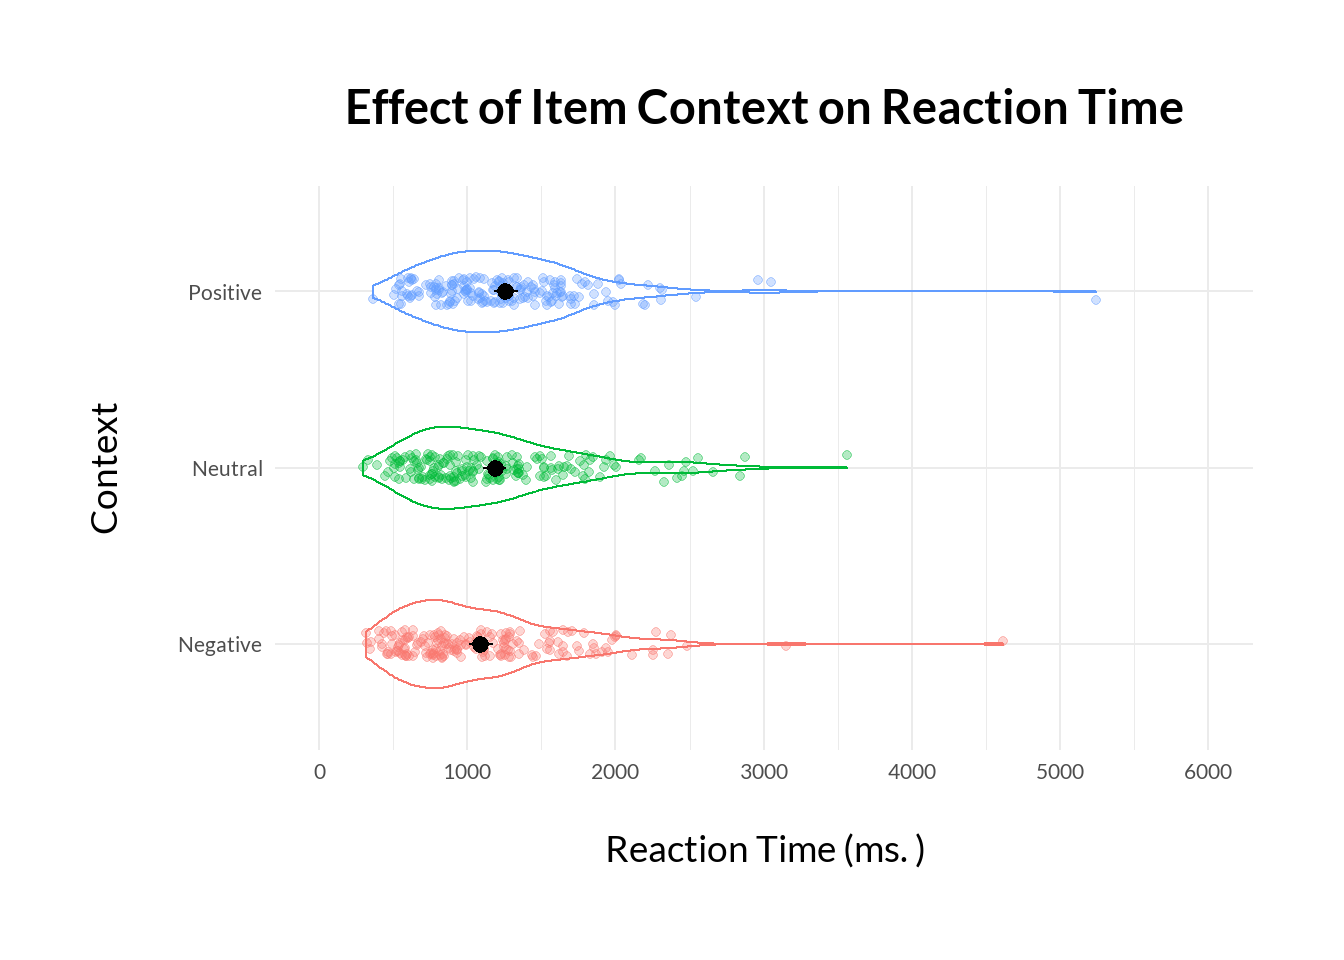
\includegraphics[width=1.8\linewidth,height=1.8\textheight]{assignment_1_markdown_files/figure-latex/unnamed-chunk-7-1}

\hypertarget{building-our-linear-model}{%
\subsection{Building our Linear Model}\label{building-our-linear-model}}

\begin{Shaded}
\begin{Highlighting}[]
\NormalTok{model }\OtherTok{\textless{}{-}} \FunctionTok{buildmer}\NormalTok{(Response\_Time }\SpecialCharTok{\textasciitilde{}}\NormalTok{ Context }\SpecialCharTok{+} 
\NormalTok{                    (}\DecValTok{1} \SpecialCharTok{+}\NormalTok{ Context }\SpecialCharTok{|}\NormalTok{ Item) }\SpecialCharTok{+}
\NormalTok{                    (}\DecValTok{1} \SpecialCharTok{+}\NormalTok{ Context }\SpecialCharTok{|}\NormalTok{ Subject),}
\NormalTok{                  q1\_data\_tidied)}
\end{Highlighting}
\end{Shaded}

\begin{verbatim}
## Determining predictor order
\end{verbatim}

\begin{verbatim}
## Fitting via lm: Response_Time ~ 1
\end{verbatim}

\begin{verbatim}
## Currently evaluating LRT for: Context
\end{verbatim}

\begin{verbatim}
## Fitting via lm: Response_Time ~ 1 + Context
\end{verbatim}

\begin{verbatim}
## Updating formula: Response_Time ~ 1 + Context
\end{verbatim}

\begin{verbatim}
## Fitting via gam, with REML: Response_Time ~ 1 + Context
\end{verbatim}

\begin{verbatim}
## Currently evaluating LRT for: 1 | Item, 1 | Subject
\end{verbatim}

\begin{verbatim}
## Fitting via lmer, with REML: Response_Time ~ 1 + Context + (1 | Item)
\end{verbatim}

\begin{verbatim}
## Fitting via lmer, with REML: Response_Time ~ 1 + Context + (1 |
##     Subject)
\end{verbatim}

\begin{verbatim}
## Updating formula: Response_Time ~ 1 + Context + (1 | Subject)
\end{verbatim}

\begin{verbatim}
## Currently evaluating LRT for: 1 | Item, Context | Subject
\end{verbatim}

\begin{verbatim}
## Fitting via lmer, with REML: Response_Time ~ 1 + Context + (1 |
##     Subject) + (1 | Item)
\end{verbatim}

\begin{verbatim}
## Fitting via lmer, with REML: Response_Time ~ 1 + Context + (1 + Context
##     | Subject)
\end{verbatim}

\begin{verbatim}
## boundary (singular) fit: see ?isSingular
\end{verbatim}

\begin{verbatim}
## Updating formula: Response_Time ~ 1 + Context + (1 | Subject) + (1 |
##     Item)
\end{verbatim}

\begin{verbatim}
## Currently evaluating LRT for: Context | Item, Context | Subject
\end{verbatim}

\begin{verbatim}
## Fitting via lmer, with REML: Response_Time ~ 1 + Context + (1 |
##     Subject) + (1 + Context | Item)
\end{verbatim}

\begin{verbatim}
## boundary (singular) fit: see ?isSingular
\end{verbatim}

\begin{verbatim}
## Fitting via lmer, with REML: Response_Time ~ 1 + Context + (1 + Context
##     | Subject) + (1 | Item)
\end{verbatim}

\begin{verbatim}
## boundary (singular) fit: see ?isSingular
\end{verbatim}

\begin{verbatim}
## Ending the ordering procedure due to having reached the maximal
##     feasible model - all higher models failed to converge. The types of
##     convergence failure are: Singular fit
\end{verbatim}

\begin{verbatim}
## Fitting ML and REML reference models
\end{verbatim}

\begin{verbatim}
## Fitting via lmer, with REML: Response_Time ~ 1 + Context + (1 |
##     Subject) + (1 | Item)
\end{verbatim}

\begin{verbatim}
## Fitting via lmer, with ML: Response_Time ~ 1 + Context + (1 | Subject)
##     + (1 | Item)
\end{verbatim}

\begin{verbatim}
## Testing terms
\end{verbatim}

\begin{verbatim}
## Fitting via lmer, with ML: Response_Time ~ 1 + (1 | Subject) + (1 |
##     Item)
\end{verbatim}

\begin{verbatim}
## Fitting via lmer, with REML: Response_Time ~ 1 + Context + (1 | Item)
\end{verbatim}

\begin{verbatim}
## Fitting via lmer, with REML: Response_Time ~ 1 + Context + (1 |
##     Subject)
\end{verbatim}

\begin{verbatim}
##   grouping    term         block      score Iteration          LRT
## 1     <NA>       1       NA NA 1         NA         1           NA
## 2     <NA> Context NA NA Context  -4.409038         1 1.186813e-03
## 3  Subject       1  NA Subject 1 -69.457193         1 5.886647e-30
## 4     Item       1     NA Item 1 -22.542847         1 1.620935e-10
\end{verbatim}

\begin{verbatim}
## All terms are significant
\end{verbatim}

\begin{verbatim}
## Finalizing by converting the model to lmerTest
\end{verbatim}

Response Time is predicted by our fixed effect of condition, plus the
random effect of our items, such that we're modelling an individual
baseline for each of our items. We're also modelling the random effect
of our subjects, such that we're modelling a different intercept for
each participant.

\begin{Shaded}
\begin{Highlighting}[]
\NormalTok{q1\_model }\OtherTok{\textless{}{-}} \FunctionTok{lmer}\NormalTok{(Response\_Time }\SpecialCharTok{\textasciitilde{}}\NormalTok{ Context }\SpecialCharTok{+} 
\NormalTok{                    (}\DecValTok{1} \SpecialCharTok{+}\NormalTok{ Context }\SpecialCharTok{|}\NormalTok{ Item) }\SpecialCharTok{+}
\NormalTok{                    (}\DecValTok{1} \SpecialCharTok{+}\NormalTok{ Context }\SpecialCharTok{|}\NormalTok{ Subject),}
\NormalTok{                  q1\_data\_tidied)}
\end{Highlighting}
\end{Shaded}

\begin{verbatim}
## boundary (singular) fit: see ?isSingular
\end{verbatim}

\begin{verbatim}
## Warning: Model failed to converge with 1 negative eigenvalue: -4.8e+00
\end{verbatim}

However, when we build this model, we're outputted with the error
message \texttt{?isSingular}. This tells us that our model that we've
build, when considering the number of parameters we're trying to
estimate, is more complex than our dataset will allow us to build. In
other words, the model that we're trying to build is too complex
relative to the richness (or lack of) (poverty??) of our dataset. We can
choose to ignore the warning, since it is not a fatal error, especially
if we had a strong theoretical reason to model all of the terms in the
random effect structure. Alternatively, we could gradually simplify the
random effects structure until we resolve the error.

Let's first drop our random slopes:

\begin{Shaded}
\begin{Highlighting}[]
\NormalTok{q1\_model }\OtherTok{\textless{}{-}} \FunctionTok{lmer}\NormalTok{(Response\_Time }\SpecialCharTok{\textasciitilde{}}\NormalTok{ Context }\SpecialCharTok{+}
\NormalTok{                   (}\DecValTok{1} \SpecialCharTok{|}\NormalTok{ Subject) }\SpecialCharTok{+}
\NormalTok{                   (}\DecValTok{1} \SpecialCharTok{|}\NormalTok{Item),}
                 \AttributeTok{data =}\NormalTok{ q1\_data\_tidied)}
\end{Highlighting}
\end{Shaded}

Now, we have a model which does has not generated the warning. Our
simpler model has response time predicted by context, whilst modelling
the random effects of subjects and items, where each subject and item
has its own baseline. However, because we've dropped modelling the
random slopes, we're assuming that the difference between the three
levels of our experimental condition are the same for all subjects and
items. This increases the likelihood of a type 1 error occurring,
leading us to think that we have an effect when one is not actually
present.

Before we move on, we should check to see whether our model adheres to
normality assumptions. To do this, we can use the
\texttt{check\_model()} function found within the
\texttt{\{performance\}} package. This will output a number of
diagnostic plots, very similar to the assumptions in the context of the
linear model, and it'll allow us to quickly tell whether our mixed model
seems to be consistent with the assumptions behind mixed models.

\begin{Shaded}
\begin{Highlighting}[]
\FunctionTok{check\_model}\NormalTok{(q1\_model)}
\end{Highlighting}
\end{Shaded}

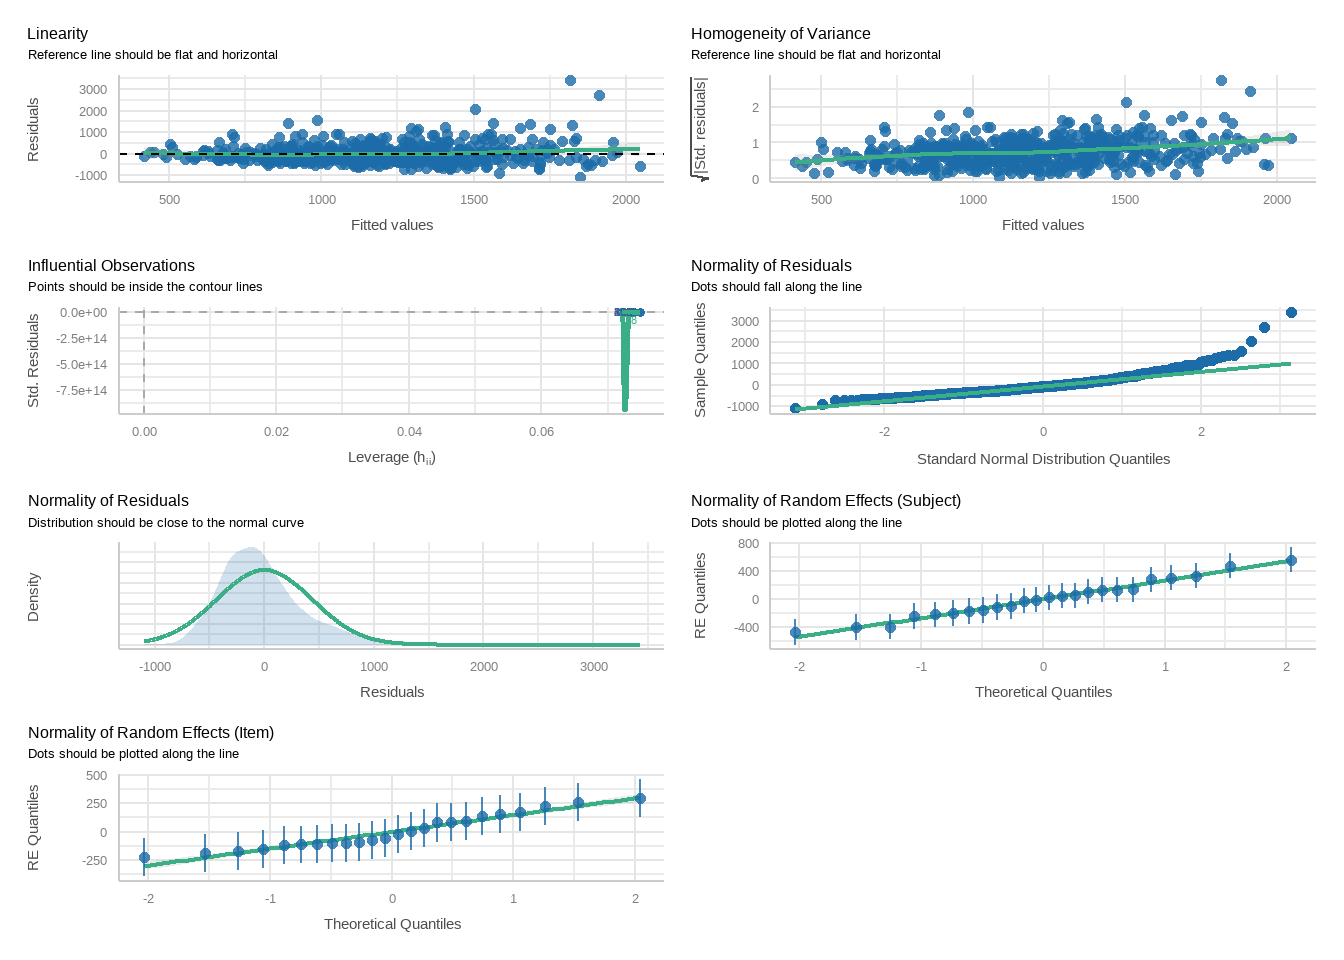
\includegraphics{assignment_1_markdown_files/figure-latex/unnamed-chunk-11-1.pdf}

Although our model seems to break down a little with its normality of
residuals, the assumptions seem mostly to have been met (``all models
are wrong, but some are useful'' - George Box).

We can ask for the output of our model using the \texttt{summary()}
function.

\begin{Shaded}
\begin{Highlighting}[]
\FunctionTok{summary}\NormalTok{(q1\_model)}
\end{Highlighting}
\end{Shaded}

\begin{verbatim}
## Linear mixed model fit by REML. t-tests use Satterthwaite's method [
## lmerModLmerTest]
## Formula: Response_Time ~ Context + (1 | Subject) + (1 | Item)
##    Data: q1_data_tidied
## 
## REML criterion at convergence: 8713.1
## 
## Scaled residuals: 
##     Min      1Q  Median      3Q     Max 
## -2.4202 -0.6259 -0.1500  0.4040  7.5278 
## 
## Random effects:
##  Groups   Name        Variance Std.Dev.
##  Subject  (Intercept)  80886   284.4   
##  Item     (Intercept)  29611   172.1   
##  Residual             206878   454.8   
## Number of obs: 574, groups:  Subject, 24; Item, 24
## 
## Fixed effects:
##                 Estimate Std. Error      df t value Pr(>|t|)    
## (Intercept)      1086.50      75.42   45.21  14.407  < 2e-16 ***
## ContextNeutral     98.28      46.55  525.13   2.111 0.035234 *  
## ContextPositive   170.80      46.49  525.09   3.674 0.000263 ***
## ---
## Signif. codes:  0 '***' 0.001 '**' 0.01 '*' 0.05 '.' 0.1 ' ' 1
## 
## Correlation of Fixed Effects:
##             (Intr) CntxtN
## ContextNtrl -0.309       
## ContextPstv -0.309  0.501
\end{verbatim}

More of the random variability can be attributed to our subjects as
oppose the the items. Critically, we are interested in our fixed
effects. For our dummy coding, \emph{R} using alphabetical information
by default when choosing a reference level of our factor against which
to compare the other levels of our factor.

which compares the Intercept (our Negative Context condition) to first
the Neutral Context condition, then to the Positive Context condition.
The average response times to our Negative condition are 1086.50 ms,
which lets us work out the average response times for the other two
conditions:

\textbf{Neutral Context condition mean:}

\begin{Shaded}
\begin{Highlighting}[]
\FunctionTok{sum}\NormalTok{(}\FloatTok{1086.5} \SpecialCharTok{+} \FloatTok{98.23}\NormalTok{)}
\end{Highlighting}
\end{Shaded}

\begin{verbatim}
## [1] 1184.73
\end{verbatim}

\textbf{Positive Context condition mean:}

\begin{Shaded}
\begin{Highlighting}[]
\FunctionTok{print}\NormalTok{(}\FloatTok{1086.5} \SpecialCharTok{+} \FloatTok{170.8}\NormalTok{)}
\end{Highlighting}
\end{Shaded}

\begin{verbatim}
## [1] 1257.3
\end{verbatim}

Our model currently has two comparisons - Negative vs Neutral, and
Negative vs Positive conditions. However, one of the issues with using
default dummy coding is that there is one comparison that has not yet
been conducted - Neutral vs Positive. As it stands, only part of the
story has emerged.

\hypertarget{likelihood-ratio-test}{%
\subsection{Likelihood Ratio Test}\label{likelihood-ratio-test}}

Let's now compare our experimental model to a model which has dropped
the fixed effect of context. First, we need to build this latter model,
which we'll call our null model. We'll use the likelihood ratio test
(LRT) to assess whether the models are statistically different from each
other. It is worth noting that models can only be compared to each other
if they are nested - it is essential that our null model is a subset of
our full factorial model, and contains the same random effects.

\begin{Shaded}
\begin{Highlighting}[]
\NormalTok{q1\_model\_null }\OtherTok{\textless{}{-}} \FunctionTok{lmer}\NormalTok{(Response\_Time }\SpecialCharTok{\textasciitilde{}} 
\NormalTok{                        (}\DecValTok{1} \SpecialCharTok{|}\NormalTok{ Subject) }\SpecialCharTok{+}
\NormalTok{                        (}\DecValTok{1} \SpecialCharTok{|}\NormalTok{ Item),}
                    \AttributeTok{data =}\NormalTok{ q1\_data\_tidied)}
\end{Highlighting}
\end{Shaded}

We can them compare our two models with the LRT within the
\texttt{anova()} function:

\begin{Shaded}
\begin{Highlighting}[]
\FunctionTok{anova}\NormalTok{(q1\_model, q1\_model\_null)}
\end{Highlighting}
\end{Shaded}

\begin{verbatim}
## Data: q1_data_tidied
## Models:
## q1_model_null: Response_Time ~ (1 | Subject) + (1 | Item)
## q1_model: Response_Time ~ Context + (1 | Subject) + (1 | Item)
##               npar    AIC    BIC  logLik deviance  Chisq Df Pr(>Chisq)   
## q1_model_null    4 8763.7 8781.1 -4377.8   8755.7                        
## q1_model         6 8754.2 8780.3 -4371.1   8742.2 13.473  2   0.001187 **
## ---
## Signif. codes:  0 '***' 0.001 '**' 0.01 '*' 0.05 '.' 0.1 ' ' 1
\end{verbatim}

If we have a look at our \emph{p}-value, we can see that our two models
differ significantly from each other (\emph{p} \textless{} .001.
Moreover, by looking at our deviance scores, the residual sums of
squares is less for our model with our fixed effects. This tells us that
our experimental manipulation seems to be making a difference.
Interestingly, the Akaike Information Criteron (AIC), which measures how
much `information' is not captured by our model, is lower in our
factorial model (i.e.~our fully factorial captures less information).
However, it is also worth noting that absolute AIC values can only be
interpreted relative to the ACI values from other models.

Following this, we run to run pairwise comparisons where we control for
the familywise error rate. We're going to use the \texttt{emmenas()}
function from the \texttt{\{emmeans\}} package to run our multiple
comparisons:

\begin{Shaded}
\begin{Highlighting}[]
\FunctionTok{emmeans}\NormalTok{(q1\_model, pairwise }\SpecialCharTok{\textasciitilde{}}\NormalTok{ Context)}
\end{Highlighting}
\end{Shaded}

\begin{verbatim}
## $emmeans
##  Context  emmean   SE   df lower.CL upper.CL
##  Negative   1087 75.4 45.2      935     1238
##  Neutral    1185 75.4 45.2     1033     1337
##  Positive   1257 75.4 45.1     1106     1409
## 
## Degrees-of-freedom method: kenward-roger 
## Confidence level used: 0.95 
## 
## $contrasts
##  contrast            estimate   SE  df t.ratio p.value
##  Negative - Neutral     -98.3 46.6 525  -2.111  0.0885
##  Negative - Positive   -170.8 46.5 525  -3.674  0.0008
##  Neutral - Positive     -72.5 46.5 525  -1.560  0.2640
## 
## Degrees-of-freedom method: kenward-roger 
## P value adjustment: tukey method for comparing a family of 3 estimates
\end{verbatim}

In this output, we get the estimates for our three experimental
conditions, as well as our pairwise comparisons, which compares our
condition with each other condition in all possible combinations. By
default, the \texttt{\{emmeans\}} function uses the Tukey corrected
comparisons method. If we correct for multiple comparisons, we see that
only one pairwise comparison is significant - Negative vs Positive
condition. The Neutral vs Positive conditions, which was significant in
the model estimates earlier, is no longer significant when taking into
account multiple comparisons.

\hypertarget{conclusion}{%
\subsection{Conclusion}\label{conclusion}}

In our model, where our experimental factor

Post hoc comparisons applying Tukey correction confirmed that words
appearing in Negative contexts resulted in significantly faster response
times than words appearing in Positive contexts (\emph{p} = .013, d =
.), but not Neutral contexts (\emph{p} = .145, d = ). The difference in
response times given for words in Neutral contexts and Positive Contexts
was not statistically significant (\emph{p} = .312, d = ).

By using a linear mixed models, we were able to model the individual
variation due to participants and items, and build up a model which is
able to take on board all of the information in our dataset. By working
over the raw data points themselves, the linear mixed model approach
uses a lot more information that is in the dataset. Finally, we can
compare different models to each other using the Likelihood Ratio Test.

\hypertarget{question-2}{%
\section{Question 2}\label{question-2}}

\begin{quote}
In a 2 x 2 repeated measures experiment, participants had to respond to
a face that depicted either ``Anger'' or ``Fear''. Each face was
presented after a Story Vignette that described either an angry or
fearful situation. There were 32 participants and 32 vignettes. Two
independent variables were manipulated within-participants in a fully
factorial design; story emotion with two levels (Anger and Fear) and
Face Expression with two levels (Anger and Fear). The time it took for
participants to respond to the face, which was taken as a measure of
reaction time, served as the dependent variable.
\end{quote}

Let's read in our data using the \texttt{\{tidyverse\}} function
\texttt{read\_csv()}:

\begin{Shaded}
\begin{Highlighting}[]
\NormalTok{q2\_data\_raw }\OtherTok{\textless{}{-}} \FunctionTok{read\_csv}\NormalTok{(}\StringTok{"assignment1\_data2.csv"}\NormalTok{)}
\end{Highlighting}
\end{Shaded}

\begin{verbatim}
## Rows: 909 Columns: 5
\end{verbatim}

\begin{verbatim}
## -- Column specification --------------------------------------------------------
## Delimiter: ","
## chr (2): StoryEmotion, FaceExpression
## dbl (3): Subject, Vignette, RT
\end{verbatim}

\begin{verbatim}
## 
## i Use `spec()` to retrieve the full column specification for this data.
## i Specify the column types or set `show_col_types = FALSE` to quiet this message.
\end{verbatim}

\begin{Shaded}
\begin{Highlighting}[]
\FunctionTok{head}\NormalTok{(q2\_data\_raw)}
\end{Highlighting}
\end{Shaded}

\begin{verbatim}
## # A tibble: 6 x 5
##   Subject Vignette StoryEmotion FaceExpression    RT
##     <dbl>    <dbl> <chr>        <chr>          <dbl>
## 1      38       10 Anger        Anger           2896
## 2      39       10 Anger        Anger           2676
## 3      40        9 Anger        Anger           1199
## 4      42       10 Anger        Anger           2464
## 5      44        9 Anger        Anger           2010
## 6      45       10 Anger        Anger           2343
\end{verbatim}

\hypertarget{data-wrangling-1}{%
\subsection{Data Wrangling}\label{data-wrangling-1}}

Like the previous question, we need to code all our columns (bar our DV)
as factors. The column titles are labelled meaningfully enough, so no
need to change them.

\begin{Shaded}
\begin{Highlighting}[]
\NormalTok{q2\_data\_tidied }\OtherTok{\textless{}{-}}\NormalTok{ q2\_data\_raw }\SpecialCharTok{\%\textgreater{}\%} 
  \FunctionTok{mutate}\NormalTok{(}\AttributeTok{Subject =} \FunctionTok{factor}\NormalTok{(Subject),}
            \AttributeTok{Vignette =} \FunctionTok{factor}\NormalTok{(Vignette),}
            \AttributeTok{StoryEmotion =} \FunctionTok{factor}\NormalTok{(StoryEmotion),}
            \AttributeTok{FaceExpression =} \FunctionTok{factor}\NormalTok{(FaceExpression))}
\FunctionTok{head}\NormalTok{(q2\_data\_tidied)}
\end{Highlighting}
\end{Shaded}

\begin{verbatim}
## # A tibble: 6 x 5
##   Subject Vignette StoryEmotion FaceExpression    RT
##   <fct>   <fct>    <fct>        <fct>          <dbl>
## 1 38      10       Anger        Anger           2896
## 2 39      10       Anger        Anger           2676
## 3 40      9        Anger        Anger           1199
## 4 42      10       Anger        Anger           2464
## 5 44      9        Anger        Anger           2010
## 6 45      10       Anger        Anger           2343
\end{verbatim}

This is much better. We can use the \texttt{str()} function to explore
our tibble in a bit more detail:

\begin{Shaded}
\begin{Highlighting}[]
\FunctionTok{str}\NormalTok{(q2\_data\_tidied)}
\end{Highlighting}
\end{Shaded}

\begin{verbatim}
## spec_tbl_df [909 x 5] (S3: spec_tbl_df/tbl_df/tbl/data.frame)
##  $ Subject       : Factor w/ 32 levels "38","39","40",..: 1 2 3 4 5 6 7 8 9 10 ...
##  $ Vignette      : Factor w/ 32 levels "1","2","3","4",..: 10 10 9 10 9 10 10 9 10 10 ...
##  $ StoryEmotion  : Factor w/ 2 levels "Anger","Fear": 1 1 1 1 1 1 1 1 1 1 ...
##  $ FaceExpression: Factor w/ 2 levels "Anger","Fear": 1 1 1 1 1 1 1 1 1 1 ...
##  $ RT            : num [1:909] 2896 2676 1199 2464 2010 ...
##  - attr(*, "spec")=
##   .. cols(
##   ..   Subject = col_double(),
##   ..   Vignette = col_double(),
##   ..   StoryEmotion = col_character(),
##   ..   FaceExpression = col_character(),
##   ..   RT = col_double()
##   .. )
##  - attr(*, "problems")=<externalptr>
\end{verbatim}

We can see that \texttt{StoryEmotion} and \texttt{FaceExpression} have
the two levels coded in.

\hypertarget{data-summarising-1}{%
\subsection{Data Summarising}\label{data-summarising-1}}

Let's generate some descriptive statistics to get an idea of what's
going on. We need to group by both of our independent variables using
the \texttt{group\_by()} function, then ask \emph{R} to work out the
mean and standard deviation of reaction time within the
\texttt{summarise()} function. Like before, we can arrange the mean
values in ascending order to see which group had the fastest reaction
times. I've mapped the outcome onto a new variable for later use in an
interaction plot.

\begin{Shaded}
\begin{Highlighting}[]
\NormalTok{q2\_descriptives }\OtherTok{\textless{}{-}}\NormalTok{ q2\_data\_tidied }\SpecialCharTok{\%\textgreater{}\%} 
  \FunctionTok{group\_by}\NormalTok{(StoryEmotion, FaceExpression) }\SpecialCharTok{\%\textgreater{}\%} 
  \FunctionTok{summarise}\NormalTok{(}\AttributeTok{mean =} \FunctionTok{mean}\NormalTok{(RT), }\AttributeTok{sd =} \FunctionTok{sd}\NormalTok{(RT)) }\SpecialCharTok{\%\textgreater{}\%} 
  \FunctionTok{arrange}\NormalTok{(mean)}
\end{Highlighting}
\end{Shaded}

\begin{verbatim}
## `summarise()` has grouped output by 'StoryEmotion'. You can override using the `.groups` argument.
\end{verbatim}

\begin{Shaded}
\begin{Highlighting}[]
\FunctionTok{head}\NormalTok{(q2\_descriptives)}
\end{Highlighting}
\end{Shaded}

\begin{verbatim}
## # A tibble: 4 x 4
## # Groups:   StoryEmotion [2]
##   StoryEmotion FaceExpression  mean    sd
##   <fct>        <fct>          <dbl> <dbl>
## 1 Anger        Anger          1848. 1079.
## 2 Fear         Fear           2028. 1163.
## 3 Fear         Anger          2525. 1867.
## 4 Anger        Fear           2634. 2025.
\end{verbatim}

Like the previous question, our output hasn't produced any NA results,
so no need to use the \texttt{\{visdat\}} function to identify the
location of missing data. At face value, it looks like participants were
quickest at identifying the facial expressions when the story preceding
it was consistent with the face emotion. Let's generate a visualisation
to get a clearer idea.

\hypertarget{data-visualisation}{%
\subsection{Data Visualisation}\label{data-visualisation}}

\begin{Shaded}
\begin{Highlighting}[]
\NormalTok{q2\_data\_tidied }\SpecialCharTok{\%\textgreater{}\%} 
  \FunctionTok{ggplot}\NormalTok{(}\FunctionTok{aes}\NormalTok{(}\AttributeTok{x =}\NormalTok{ StoryEmotion}\SpecialCharTok{:}\NormalTok{FaceExpression, }\AttributeTok{y =}\NormalTok{ RT, }\AttributeTok{colour =}\NormalTok{ FaceExpression)) }\SpecialCharTok{+}
  \FunctionTok{geom\_violin}\NormalTok{() }\SpecialCharTok{+}
  \FunctionTok{geom\_point}\NormalTok{(}\AttributeTok{alpha =} \FloatTok{0.2}\NormalTok{, }\AttributeTok{position =} \FunctionTok{position\_jitter}\NormalTok{(}\AttributeTok{width =} \FloatTok{0.1}\NormalTok{, }\AttributeTok{seed =} \DecValTok{42}\NormalTok{)) }\SpecialCharTok{+}
  \FunctionTok{stat\_summary}\NormalTok{(}\AttributeTok{fun.data =} \StringTok{\textquotesingle{}mean\_cl\_boot\textquotesingle{}}\NormalTok{, }\AttributeTok{colour =} \StringTok{\textquotesingle{}black\textquotesingle{}}\NormalTok{) }\SpecialCharTok{+}
  \FunctionTok{theme\_minimal}\NormalTok{() }\SpecialCharTok{+}
  \FunctionTok{scale\_y\_continuous}\NormalTok{(}\AttributeTok{breaks =} \FunctionTok{seq}\NormalTok{(}\DecValTok{0}\NormalTok{, }\DecValTok{10000}\NormalTok{, }\AttributeTok{by =} \DecValTok{1250}\NormalTok{),}
                     \AttributeTok{limits =} \FunctionTok{c}\NormalTok{(}\DecValTok{0}\NormalTok{, }\DecValTok{10000}\NormalTok{)) }\SpecialCharTok{+}
  \FunctionTok{scale\_x\_discrete}\NormalTok{(}\AttributeTok{labels =} \FunctionTok{c}\NormalTok{(}\StringTok{"Anger:Anger"} \OtherTok{=} \StringTok{"Anger"}\NormalTok{,}
                              \StringTok{"Anger:Fear"} \OtherTok{=} \StringTok{"Anger"}\NormalTok{,}
                              \StringTok{"Fear:Anger"} \OtherTok{=} \StringTok{"Fear"}\NormalTok{,}
                              \StringTok{"Fear:Fear"} \OtherTok{=} \StringTok{"Fear"}\NormalTok{)) }\SpecialCharTok{+}
  \FunctionTok{labs}\NormalTok{(}\AttributeTok{x =} \StringTok{"Story Emotion"}\NormalTok{,}
       \AttributeTok{y =} \StringTok{"Reaction Time (ms. )"}\NormalTok{,}
       \AttributeTok{title =} \StringTok{"Examining the Effect of Story Emotion}\SpecialCharTok{\textbackslash{}n}\StringTok{ and Face Expression on Reaction Time"}\NormalTok{) }\SpecialCharTok{+}
  \FunctionTok{theme}\NormalTok{(}\AttributeTok{plot.title =} \FunctionTok{element\_text}\NormalTok{(}\AttributeTok{size =} \DecValTok{40}\NormalTok{, }\AttributeTok{hjust =} \FloatTok{0.5}\NormalTok{, }\AttributeTok{margin =} \FunctionTok{margin}\NormalTok{(}\AttributeTok{b =} \DecValTok{15}\NormalTok{), }\AttributeTok{line =} \FloatTok{0.5}\NormalTok{, }\AttributeTok{face =} \StringTok{"bold"}\NormalTok{),}
        \AttributeTok{axis.title.x =} \FunctionTok{element\_text}\NormalTok{(}\AttributeTok{size =} \DecValTok{30}\NormalTok{, }\AttributeTok{margin =} \FunctionTok{margin}\NormalTok{(}\AttributeTok{t =} \DecValTok{20}\NormalTok{)),}
        \AttributeTok{axis.title.y =} \FunctionTok{element\_text}\NormalTok{(}\AttributeTok{size =} \DecValTok{30}\NormalTok{, }\AttributeTok{margin =} \FunctionTok{margin}\NormalTok{(}\AttributeTok{r =} \DecValTok{20}\NormalTok{)),}
        \AttributeTok{text =} \FunctionTok{element\_text}\NormalTok{(}\AttributeTok{family =} \StringTok{"lato"}\NormalTok{, }\AttributeTok{size =} \DecValTok{25}\NormalTok{)) }\SpecialCharTok{+}
  \FunctionTok{coord\_flip}\NormalTok{()}
\end{Highlighting}
\end{Shaded}

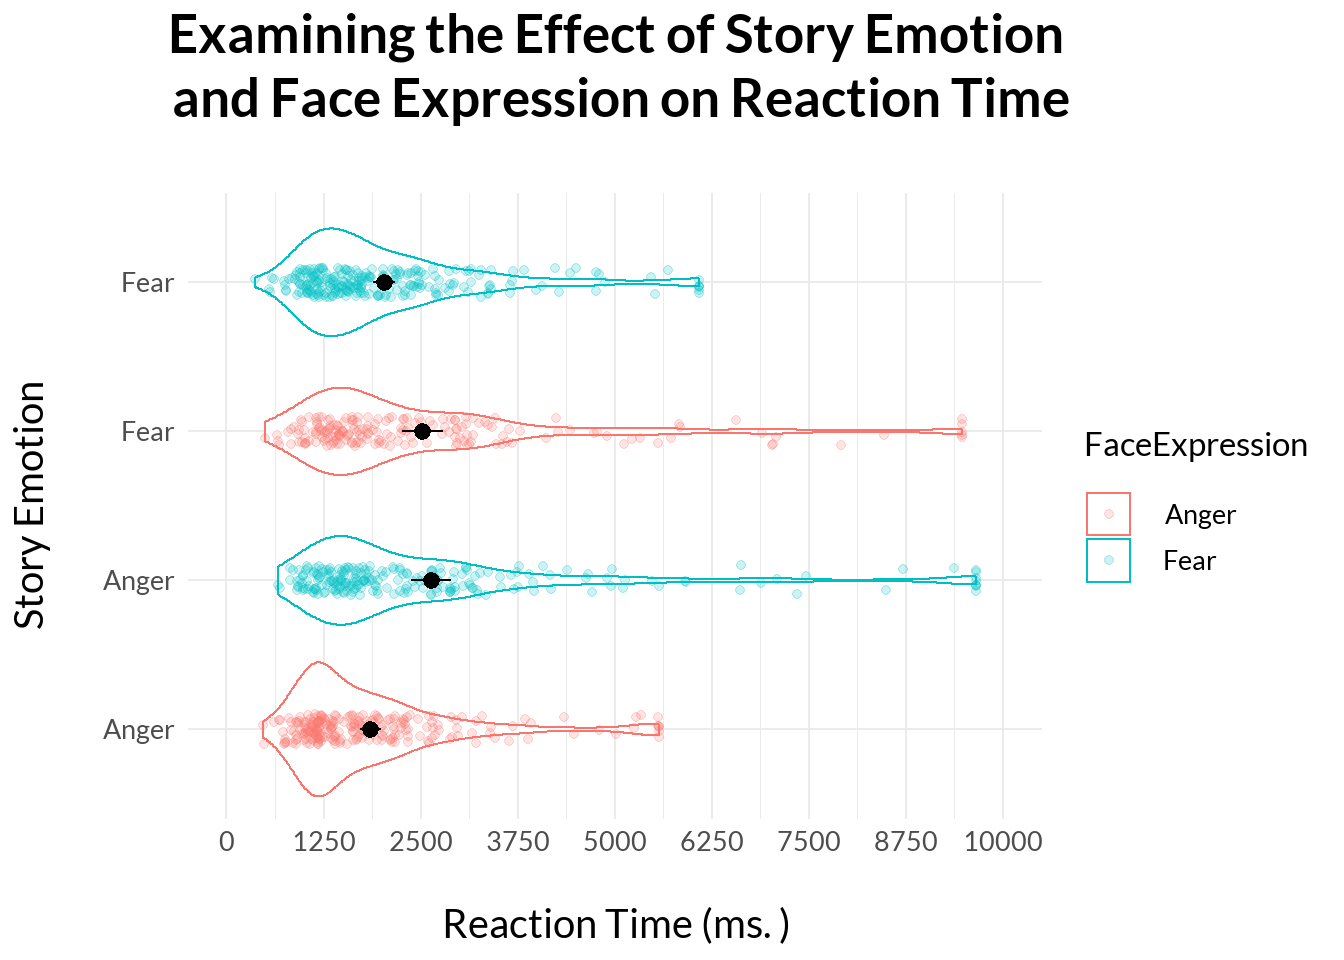
\includegraphics{assignment_1_markdown_files/figure-latex/unnamed-chunk-22-1.pdf}

\begin{Shaded}
\begin{Highlighting}[]
\NormalTok{q2\_data\_tidied }\SpecialCharTok{\%\textgreater{}\%} 
  \FunctionTok{ggplot}\NormalTok{(}\FunctionTok{aes}\NormalTok{(}\AttributeTok{x =}\NormalTok{ StoryEmotion}\SpecialCharTok{:}\NormalTok{FaceExpression, }\AttributeTok{y =}\NormalTok{ RT, }\AttributeTok{colour =}\NormalTok{ FaceExpression)) }\SpecialCharTok{+}
  \FunctionTok{geom\_violin}\NormalTok{(}\AttributeTok{width =} \FloatTok{0.6}\NormalTok{) }\SpecialCharTok{+}
  \FunctionTok{geom\_point}\NormalTok{(}\AttributeTok{alpha =} \FloatTok{0.2}\NormalTok{, }\AttributeTok{position =} \FunctionTok{position\_jitter}\NormalTok{(}\AttributeTok{width =} \FloatTok{0.1}\NormalTok{, }\AttributeTok{seed =} \DecValTok{42}\NormalTok{)) }\SpecialCharTok{+}
  \FunctionTok{stat\_summary}\NormalTok{(}\AttributeTok{fun.data =} \StringTok{\textquotesingle{}mean\_cl\_boot\textquotesingle{}}\NormalTok{, }\AttributeTok{colour =} \StringTok{\textquotesingle{}black\textquotesingle{}}\NormalTok{) }\SpecialCharTok{+}
  \FunctionTok{theme\_minimal}\NormalTok{() }\SpecialCharTok{+}
  \FunctionTok{scale\_y\_continuous}\NormalTok{(}\AttributeTok{breaks =} \FunctionTok{seq}\NormalTok{(}\DecValTok{0}\NormalTok{, }\DecValTok{10000}\NormalTok{, }\AttributeTok{by =} \DecValTok{1250}\NormalTok{),}
                     \AttributeTok{limits =} \FunctionTok{c}\NormalTok{(}\DecValTok{0}\NormalTok{, }\DecValTok{10000}\NormalTok{)) }\SpecialCharTok{+}
  \FunctionTok{scale\_x\_discrete}\NormalTok{(}\AttributeTok{labels =} \FunctionTok{c}\NormalTok{(}\StringTok{"Anger:Anger"} \OtherTok{=} \StringTok{"Anger"}\NormalTok{,}
                              \StringTok{"Anger:Fear"} \OtherTok{=} \StringTok{"Anger"}\NormalTok{,}
                              \StringTok{"Fear:Anger"} \OtherTok{=} \StringTok{"Fear"}\NormalTok{,}
                              \StringTok{"Fear:Fear"} \OtherTok{=} \StringTok{"Fear"}\NormalTok{)) }\SpecialCharTok{+}
  \FunctionTok{labs}\NormalTok{(}\AttributeTok{x =} \StringTok{"Story Emotion"}\NormalTok{,}
       \AttributeTok{y =} \StringTok{"Reaction Time (ms. )"}\NormalTok{,}
       \AttributeTok{title =} \StringTok{"Examining the Effect of Story Emotion}\SpecialCharTok{\textbackslash{}n}\StringTok{ and Face Expression on Reaction Time"}\NormalTok{) }\SpecialCharTok{+}
  \FunctionTok{coord\_flip}\NormalTok{()}
\end{Highlighting}
\end{Shaded}

\includegraphics{assignment_1_markdown_files/figure-latex/unnamed-chunk-23-1.pdf}

We can also build an interaction plot to get an idea of any interactions
that may be present. First, we'll bring the legend closer to the lines
by creating a new dataset that includes the y-values of the points where
both lines end. We also need the labels that will be at the end of the
lines. For this we use the function \texttt{case\_when()}.

\begin{Shaded}
\begin{Highlighting}[]
\NormalTok{labels }\OtherTok{\textless{}{-}}\NormalTok{ q2\_descriptives }\SpecialCharTok{\%\textgreater{}\%} 
  \FunctionTok{filter}\NormalTok{(StoryEmotion }\SpecialCharTok{==} \StringTok{"Fear"}\NormalTok{) }\SpecialCharTok{\%\textgreater{}\%} 
  \FunctionTok{mutate}\NormalTok{(}\AttributeTok{label =} \FunctionTok{case\_when}\NormalTok{(FaceExpression }\SpecialCharTok{==} \StringTok{"Anger"} \SpecialCharTok{\textasciitilde{}} \StringTok{"Angry Face}\SpecialCharTok{\textbackslash{}n}\StringTok{ Expression"}\NormalTok{,}
\NormalTok{                           FaceExpression }\SpecialCharTok{==} \StringTok{"Fear"} \SpecialCharTok{\textasciitilde{}} \StringTok{"Fearful Face}\SpecialCharTok{\textbackslash{}n}\StringTok{ Expressions"}\NormalTok{))}
\FunctionTok{head}\NormalTok{(labels)}
\end{Highlighting}
\end{Shaded}

\begin{verbatim}
## # A tibble: 2 x 5
## # Groups:   StoryEmotion [1]
##   StoryEmotion FaceExpression  mean    sd label                       
##   <fct>        <fct>          <dbl> <dbl> <chr>                       
## 1 Fear         Fear           2028. 1163. "Fearful Face\n Expressions"
## 2 Fear         Anger          2525. 1867. "Angry Face\n Expression"
\end{verbatim}

Using the \texttt{descriptive\_stats} dataset we created earlier, we can
add the geom\_text to our interaction plot and pass our dataset
\texttt{labels} to the geom. Among the aesthetics, \texttt{geom\_text()}
includes the aesthetic label, which stands for the text we will add to
the visualization. We've also scaled down the y-axis using the
\texttt{scale\_y\_continuous()} function to visually increase the
distance between the means, aiding interpretation.

\begin{Shaded}
\begin{Highlighting}[]
\NormalTok{q2\_descriptives }\SpecialCharTok{\%\textgreater{}\%} 
  \FunctionTok{ggplot}\NormalTok{(}\FunctionTok{aes}\NormalTok{(}\AttributeTok{x =}\NormalTok{ StoryEmotion, }\AttributeTok{y =}\NormalTok{ mean)) }\SpecialCharTok{+}
  \FunctionTok{geom\_line}\NormalTok{(}\AttributeTok{size =} \FloatTok{1.2}\NormalTok{, }\FunctionTok{aes}\NormalTok{(}\AttributeTok{group =}\NormalTok{ FaceExpression, }\AttributeTok{colour =}\NormalTok{ FaceExpression)) }\SpecialCharTok{+}
  \FunctionTok{geom\_point}\NormalTok{(}\AttributeTok{size =} \FloatTok{2.6}\NormalTok{, }\FunctionTok{aes}\NormalTok{(}\AttributeTok{colour =}\NormalTok{ FaceExpression), }\AttributeTok{shape =} \DecValTok{15}\NormalTok{) }\SpecialCharTok{+}
  \FunctionTok{geom\_text}\NormalTok{(}\AttributeTok{size =} \FloatTok{6.5}\NormalTok{, }\FunctionTok{aes}\NormalTok{(}\AttributeTok{label =}\NormalTok{ label,}
                          \AttributeTok{colour =}\NormalTok{ FaceExpression),}
            \AttributeTok{data =}\NormalTok{ labels,}
            \AttributeTok{nudge\_x =} \FloatTok{0.12}\NormalTok{,}
            \AttributeTok{nudge\_y =} \DecValTok{80}\NormalTok{) }\SpecialCharTok{+}
  \FunctionTok{guides}\NormalTok{(}\AttributeTok{colour =} \StringTok{\textquotesingle{}none\textquotesingle{}}\NormalTok{) }\SpecialCharTok{+}
  \FunctionTok{scale\_y\_continuous}\NormalTok{(}\AttributeTok{breaks =} \FunctionTok{seq}\NormalTok{(}\DecValTok{1800}\NormalTok{, }\DecValTok{2800}\NormalTok{, }\AttributeTok{by =} \DecValTok{200}\NormalTok{),}
                     \AttributeTok{limits =} \FunctionTok{c}\NormalTok{(}\DecValTok{1800}\NormalTok{, }\DecValTok{2800}\NormalTok{)) }\SpecialCharTok{+}
  \FunctionTok{labs}\NormalTok{(}\AttributeTok{x =} \StringTok{"Story Emotion"}\NormalTok{,}
       \AttributeTok{y =} \StringTok{"Reaction Time (ms. )"}\NormalTok{,}
       \AttributeTok{title =} \StringTok{"Examining the Interaction Between }
\StringTok{       Story Emotion and Face Expression"}\NormalTok{) }\SpecialCharTok{+}
  \FunctionTok{theme\_minimal}\NormalTok{() }\SpecialCharTok{+}
  \FunctionTok{theme}\NormalTok{(}\AttributeTok{text =} \FunctionTok{element\_text}\NormalTok{(}\AttributeTok{family =} \StringTok{"lato"}\NormalTok{, }\AttributeTok{size =} \DecValTok{26}\NormalTok{),}
        \AttributeTok{plot.title =} \FunctionTok{element\_text}\NormalTok{(}\AttributeTok{size =} \DecValTok{30}\NormalTok{, }\AttributeTok{hjust =} \FloatTok{0.5}\NormalTok{, }\AttributeTok{margin =} \FunctionTok{margin}\NormalTok{(}\AttributeTok{b =} \DecValTok{35}\NormalTok{), }\AttributeTok{face =} \StringTok{"bold"}\NormalTok{),}
        \AttributeTok{axis.title.x =} \FunctionTok{element\_text}\NormalTok{(}\AttributeTok{size =} \DecValTok{30}\NormalTok{, }\AttributeTok{margin =} \FunctionTok{margin}\NormalTok{(}\AttributeTok{t =} \DecValTok{30}\NormalTok{)),}
        \AttributeTok{axis.title.y =} \FunctionTok{element\_text}\NormalTok{(}\AttributeTok{size =} \DecValTok{30}\NormalTok{, }\AttributeTok{margin =} \FunctionTok{margin}\NormalTok{(}\AttributeTok{r =} \DecValTok{30}\NormalTok{)),}
        \AttributeTok{plot.margin =} \FunctionTok{unit}\NormalTok{(}\FunctionTok{rep}\NormalTok{(}\FloatTok{1.2}\NormalTok{, }\DecValTok{4}\NormalTok{), }\StringTok{"cm"}\NormalTok{))}
\end{Highlighting}
\end{Shaded}

\includegraphics[width=1.8\linewidth,height=1.8\textheight]{assignment_1_markdown_files/figure-latex/unnamed-chunk-25-1}

We can see here that we have a crossover interaction as the polarity of
the difference flips. The graph shows that Reaction Time was faster for
Angry Face Expressions when the preceding story was also angry.
Likewise, Reaction Time was faster for Fearful Face Expressions when the
preceding story was also Fearful. Due to our crossover interaction, it
is unlikely that we'll have significant main effects of \emph{both}
Story Emotion and Face Expression variables, but a significant
interaction effect is likely.

\end{document}
